\section{Description of Data}
% 最も一般的な予測タスクは,
% 実数値の$n$次元の特徴ベクトル$\vtr{x} \in \R^{n}$から目標$T$
% (2値分類であれば$T = \{ +, - \}$,回帰であれば$T = \R$)
% への関数$y : \R^{n} \to T$を推定することである.
データ$D = \{ ( \vtr{x}^{(1)}, y^{(1)} ), ( \vtr{x}^{(2)}, y^{(2)} ), \cdots  \}$
があるものとする.

FMでは,入力ベクトル$\vtr{x}$は非常にスパースであるものとする.
ここで,$m(\vtr{x})$をベクトル$\vtr{x}$の非ゼロ成分の数,
$\overline{m}_{D}$を全てのベクトル$\vtr{x} \in D$の非ゼロ成分の数$m(\vtr{x})$の平均とする.

実世界には,$\overline{m}_{D} \ll n$となるような非常にスパースなデータがよくある.
例えば,購買履歴データであったり,テキスト処理におけるBag of Wordsデータなどである.
また,e-Learningのログデータもスパースなデータのひとつである.
このようにデータがスパースになってしまうひとつの理由として,
カテゴリ変数\footnote{ユーザー,アイテム,性別,単語など有限のラベルに分けられるもの.
カテゴリ変数以外に,離散変数,連続変数がある.}
を多く用いることが挙げられる.
カテゴリ変数はOne-Hot Encodingをして使用することが多いため,スパースになりやすい.
\begin{figure}[H]
  \centering
  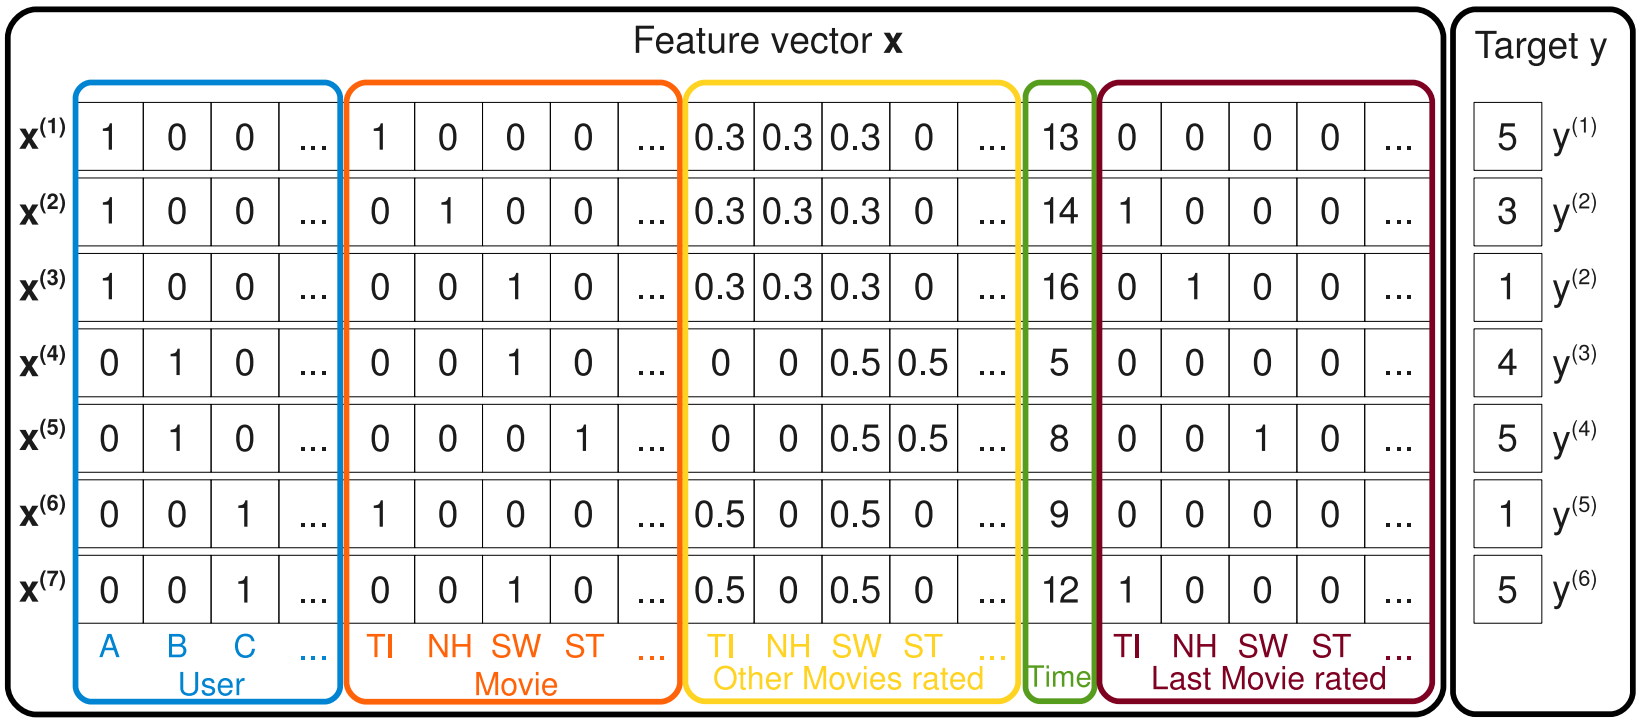
\includegraphics[width=0.85\hsize, bb=0 0 1640 720]{fig/FM_data.png}
  \caption{データ例}
  \label{fig:data}
\end{figure}
